\documentclass[11pt,a4paper]{article}
\usepackage[a4paper,top=11mm,bottom=10mm,left=14mm,right=14mm]{geometry}
\usepackage[T1]{fontenc}
\usepackage{amsmath}
\usepackage{amssymb}
\usepackage{enumitem}
\usepackage{multicol}
\usepackage{array}
\usepackage{xcolor}
\usepackage{tikz}
\usepackage[most]{tcolorbox}
\usetikzlibrary{arrows.meta,matrix}

% ================================================================
% Challenge: ratio and the shape of A4 paper.
%
% A four-page challenge sheet on ratio for confident pupils who know
% Pythagoras' theorem and surds. The quadratic equations are solved by
% rearranging a completed-square form that the sheet gives as a fact, so
% the quadratic formula is not needed. It is built on
% one idea: when a shape is cut into pieces that are similar to the
% whole shape, the rule for cutting it fixes the ratio of its lengths.
% Similar rectangles have equivalent ratios short : long, so the method
% throughout is to write both ratios in the form 1 : n and set them
% equal. Equivalent ratios and equations are both worked with curved
% arrows that show the same operation done to both sides.
%
% The first pages are discovery. The key idea box shows folding, similar
% shapes and equivalent ratios in pictures. Q1 writes scale drawings of
% A3, A4 and A5 in the form 1 : n. Q2 folds other rectangles in half,
% and finds the two that the shape that stays the same lies between. Q3
% practises equivalent ratios, and shows that the second part divided
% by the first part is the same for equivalent ratios. Q4 is open:
% pupils set up and solve the equation for 1 : sqrt(2) themselves, with
% only the hint that the whole and half sheets have equivalent ratios.
%
% Part 1 (Q5 to Q8) uses the ratio with real paper: US Letter, the sizes
% A0 to A6, photocopier percentages, and a fold that shows the ratio on
% a real sheet.
%
% Part 2 changes the rule: three strips (Q9, the method of Q4 again, with
% the picture and lines for the two ratios but no other scaffold), then
% n strips, the golden rectangle (one square cut off) and the silver
% rectangle (a square cut off A4).
% Q13 moves to triangles and an L-shape, and asks why n similar pieces
% always give 1 : sqrt(n).
%
% Page 4 goes into more dimensions: a box that halves into two similar
% boxes is 1 : cbrt(2) : cbrt(4) (Q14), and the four-dimensional box is
% 1 : 2^(1/4) : 2^(1/2) : 2^(3/4) (Q15). Q16 collects the pattern and
% asks what happens as the number of dimensions grows. Q17 is the
% A-series spiral and the sum 1/2 + 1/4 + 1/8 + ... = 1. Q18 is the
% family x^2 - kx - 1 = 0, solved from its completed-square form, and an
% open task.
%
% There is little working space, so pupils work on paper. The answers
% are in a comment beside each question.
% ================================================================

\pagestyle{empty}
\linespread{1.04}\selectfont
\setlength{\parskip}{3pt}
\setlength{\parindent}{0pt}
\renewcommand{\arraystretch}{1.25}
\setlist[enumerate,1]{label=\textbf{Q\arabic*.}, leftmargin=*, itemsep=6pt,
  topsep=2pt, partopsep=0pt, parsep=2pt}
\setlist[enumerate,2]{label=(\alph*), leftmargin=*, itemsep=2pt, topsep=2pt,
  partopsep=0pt, parsep=1pt}
\setlength{\multicolsep}{2pt}

% Gaps to write in: \gap inside a sentence, \tgap inside a table,
% \eqgap inside a ratio or an equation, and \opgap for an operation
% beside a curved arrow. \gapstrut makes a table row tall enough to
% write in.
\newcommand{\ansline}[1][2.2cm]{\underline{\hspace{#1}}}
\newcommand{\gap}{\ansline[1.1cm]}
\newcommand{\tgap}{\ansline[0.8cm]}
\newcommand{\eqgap}{\underline{\hspace{1.0cm}}}
\newcommand{\opgap}{\underline{\hspace{0.55cm}}}
\newcommand{\gapstrut}{\rule[-2mm]{0pt}{7mm}}

% The idea the sheet is built on, in a box that is tinted only faintly
% so that the printed sheet uses little toner.
\newtcolorbox{keyidea}{colback=orange!3,colframe=orange!35,boxrule=0.6pt,
  left=6pt,right=6pt,top=2pt,bottom=2pt}

% The part headings: a thick rule, the title and a thin rule.
\newcommand{\parttitle}[2]{%
  \par\vspace{4pt}%
  {\color{blue!45!black}\hrule height 1pt}\vspace{3pt}%
  {\large\bfseries Part #1: #2\par}\vspace{2pt}%
  {\color{blue!45!black}\hrule height 0.4pt}\vspace{3pt}}

% A small bold title above a working.
\newcommand{\worktitle}[1]{{\small\bfseries #1}\par\vspace{1pt}}

% Doing the same thing to both sides, for an equation or for the parts
% of a ratio. The lines are the rows of a matrix, lined up on the equals
% sign or the colon, and a curved arrow on each side goes from one line
% to the next, with the operation beside it. The operations are a list,
% one for each step:
%   \bothsides{x \& = \& \dfrac{2}{x}\\ x^2 \& = \& 2\\}{\times x}
%   \bothsides{0.75 \& : \& 1\\ 1 \& : \& 1.333\\}{\div0.75}
% A ratio with three parts uses the option ratio3:
%   \bothsides[ratio3]{a \& : \& b \& : \& c\\ ...}{...}
% An operation given as \opgap is left for pupils to write in.
\tikzset{
  bsline/.style  = {matrix of math nodes, ampersand replacement=\&,
                    row sep=0.55em, column sep=0.2em,
                    nodes={inner sep=1pt},
                    column 1/.style={anchor=base east},
                    column 2/.style={anchor=base},
                    column 3/.style={anchor=base west}},
  ratio3/.style  = {column 3/.style={anchor=base},
                    column 4/.style={anchor=base},
                    column 5/.style={anchor=base west}},
  bsarrow/.style = {-{Stealth[length=4pt]}, blue!55!black, semithick},
  bslab/.style   = {font=\small, text=blue!55!black, inner sep=1.5pt},
}
\newcommand{\bothsides}[3][]{%
  \begin{tikzpicture}[baseline=(m-1-2.base)]
    \matrix (m) [bsline, #1] {#2};
    \foreach \op [count=\i, evaluate=\i as \j using int(\i+1)] in {#3} {
      \draw[bsarrow] ([xshift=-3pt]m.west |- m-\i-2.center) to[bend right=50]
        node[bslab, left] {$\op$} ([xshift=-3pt]m.west |- m-\j-2.center);
      \draw[bsarrow] ([xshift=3pt]m.east |- m-\i-2.center) to[bend left=50]
        node[bslab, right] {$\op$} ([xshift=3pt]m.east |- m-\j-2.center);
    }
  \end{tikzpicture}}

% A rectangle with short side 1 and long side n, cut into k equal strips
% across its long side, with one strip drawn beside it.
%   \cutdiagram{k}{n}{label of the long side}{label of a strip's short side}{word}
\newcolumntype{C}[1]{>{\centering\arraybackslash}p{#1}}
\newcommand{\cutdiagram}[5]{%
  \begin{tikzpicture}[baseline=(current bounding box.north), font=\small]
    \pgfmathsetmacro{\sw}{1.0}
    \pgfmathsetmacro{\lh}{1.0*#2}
    \pgfmathsetmacro{\st}{\lh/#1}
    \draw[thick, fill=blue!3] (0,0) rectangle (\sw,\lh);
    \foreach \k in {1,...,#1} {\ifnum\k<#1
      \draw[dashed] (0,\k*\st) -- (\sw,\k*\st);\fi}
    \node[below] at (\sw/2,0) {$1$};
    \node[left] at (0,\lh/2) {#3};
    \draw[-{Stealth[length=4pt]}, gray] (\sw+0.1,\lh/2) --
      node[above, font=\scriptsize, text=black] {#5} (\sw+0.7,\lh/2);
    \draw[thick, fill=blue!3] (\sw+1.55,\lh/2-\st/2) rectangle
      (2*\sw+1.55,\lh/2+\st/2);
    \node[below] at (1.5*\sw+1.55,\lh/2-\st/2) {$1$};
    \node[left] at (\sw+1.55,\lh/2) {#4};
  \end{tikzpicture}}

% A scale drawing of a sheet of paper at 1 : 20, with its name inside and
% its sides labelled in millimetres. Every drawing has the same height,
% so that drawings of different sizes stand on the same line.
%   \papersheet{short side in mm}{long side in mm}{name}
\newcommand{\papersheet}[3]{%
  \begin{tikzpicture}[font=\small]
    \path (0,-0.4) -- (0,2.15);
    \draw[thick, fill=blue!3] (0,0) rectangle (#1/200,#2/200);
    \node[font=\scriptsize] at (#1/400,#2/400) {#3};
    \node[below, font=\scriptsize] at (#1/400,0) {$#1$\,mm};
    \node[left, font=\scriptsize] at (0,#2/400) {$#2$\,mm};
  \end{tikzpicture}}

% One of the rectangles in Q2: the whole sheet, the working that writes
% the half sheet in the form 1 : n, and whether the shape is the same.
%   \foldcell{whole sheet ratio}{working}{answer or gap}
\newcommand{\foldcell}[3]{%
  \begin{minipage}[t]{0.48\linewidth}
  \centering
  \worktitle{Whole sheet $#1$. Half sheet, short : long:}
  #2\hspace{0.8em}{\small Same shape?\ \ #3}
  \end{minipage}}

\begin{document}

% ================================================================
% PAGE 1: discovering 1 : sqrt(2)
% ================================================================

\begin{center}
  {\Large\bfseries Challenge: Ratio and the Shape of A4 Paper}
\end{center}
\vspace{-6pt}

\begin{keyidea}
\small
\begin{minipage}[t]{0.35\linewidth}
\centering
\textbf{Folding}\par\vspace{4pt}
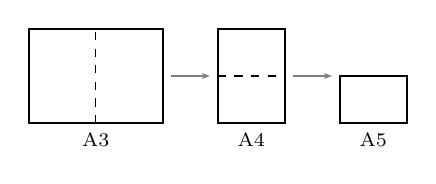
\begin{tikzpicture}[font=\scriptsize]
  \draw[thick, fill=white] (0,0) rectangle (1.7,1.2);
  \draw[dashed] (0.85,0) -- (0.85,1.2);
  \node[below] at (0.85,0) {A3};
  \draw[-{Stealth[length=3pt]}, gray] (1.8,0.6) -- (2.3,0.6);
  \draw[thick, fill=white] (2.4,0) rectangle (3.25,1.2);
  \draw[dashed] (2.4,0.6) -- (3.25,0.6);
  \node[below] at (2.825,0) {A4};
  \draw[-{Stealth[length=3pt]}, gray] (3.35,0.6) -- (3.85,0.6);
  \draw[thick, fill=white] (3.95,0) rectangle (4.8,0.6);
  \node[below] at (4.375,0) {A5};
\end{tikzpicture}\par\vspace{2pt}
{\footnotesize Folding a sheet in half halves its long side, and makes the
next size.}
\end{minipage}\hfill
\begin{minipage}[t]{0.29\linewidth}
\centering
\textbf{Similar shapes}\par\vspace{4pt}
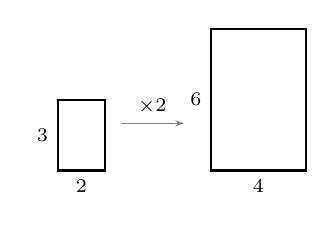
\begin{tikzpicture}[font=\scriptsize]
  \draw[thick, fill=white] (0,0) rectangle (0.6,0.9);
  \node[below] at (0.3,0) {$2$};
  \node[left] at (0,0.45) {$3$};
  \draw[-{Stealth[length=3pt]}, gray] (0.8,0.6) --
    node[above, text=black] {$\times2$} (1.6,0.6);
  \draw[thick, fill=white] (1.95,0) rectangle (3.15,1.8);
  \node[below] at (2.55,0) {$4$};
  \node[left] at (1.95,0.9) {$6$};
\end{tikzpicture}\par\vspace{2pt}
{\footnotesize An enlargement: every length is multiplied by the same scale
factor.}
\end{minipage}\hfill
\begin{minipage}[t]{0.31\linewidth}
\centering
\textbf{Equivalent ratios}\par\vspace{6pt}
\bothsides{4 \& : \& 6\\ 2 \& : \& 3\\ 1 \& : \& 1.5\\}{\div2, \div2}
\par\vspace{4pt}
{\footnotesize Multiply or divide both parts by the same number. The form
$1:n$ makes ratios easy to compare.}
\end{minipage}

\vspace{4pt}
\centering
\textbf{Similar rectangles have equivalent ratios} short side : long side.
\end{keyidea}

\begin{enumerate}

% Answers: A4 210 : 297 = 1 : 1.414 (divide by 210). A5 148 : 210 =
% 1 : 1.419 (divide by 148). (b) All three are about 1 : 1.41: the
% sheets are (very nearly) similar.
\item
\begin{enumerate}
  \item The scale drawings ($1:20$) show three sheets of paper. Write each
        as short : long in the form $1:n$, to 3 decimal places.

        \vspace{2pt}
        \begin{minipage}[t]{0.32\linewidth}
        \centering
        \papersheet{297}{420}{A3}\par\vspace{2pt}
        \bothsides{297 \& : \& 420\\ 1 \& : \& 1.414\\}{\div297}
        \end{minipage}\hfill
        \begin{minipage}[t]{0.32\linewidth}
        \centering
        \papersheet{210}{297}{A4}\par\vspace{2pt}
        \bothsides{210 \& : \& 297\\ 1 \& : \& \eqgap\\}{\div210}
        \end{minipage}\hfill
        \begin{minipage}[t]{0.32\linewidth}
        \centering
        \papersheet{148}{210}{A5}\par\vspace{2pt}
        \bothsides{148 \& : \& 210\\ 1 \& : \& \eqgap\\}{\opgap}
        \end{minipage}
  \item What do you notice?
\end{enumerate}

% Answers: (a) 1 : 2: half 1 : 1, divide by 1, 1 : 1 (a square), no.
% 1 : 1.2: half 0.6 : 1, divide by 0.6, 1 : 1.667, no.
% 1 : 1.4: half 0.7 : 1, divide by 0.7, 1 : 1.429, no.
% (b) Between 1 : 1.4 and 1 : 1.5. For 1 : 1.4 the half sheet is
% 1 : 1.429, more than 1.4; for 1 : 1.5 it is 1 : 1.333, less than 1.5.
\item
\begin{minipage}[t]{0.70\linewidth}
Not every rectangle keeps its shape when it is folded in half. Folding a sheet
halves its long side, as in the diagram.
\begin{enumerate}
  \item Fill in the gaps to write each half sheet as short : long in the form
        $1:n$. Is the half sheet the same shape as the whole sheet?
\end{enumerate}
\end{minipage}\hfill
\begin{minipage}[t]{0.27\linewidth}
\vspace{0pt}
\centering
\cutdiagram{2}{1.5}{$1.5$}{$0.75$}{fold}
\end{minipage}

\vspace{4pt}
\foldcell{1:1.5}{\bothsides{0.75 \& : \& 1\\ 1 \& : \& 1.333\\}{\div0.75}}{No}%
\hfill
\foldcell{1:2}{\bothsides{\eqgap \& : \& 1\\ 1 \& : \& \eqgap\\}{\div1}}{\tgap}

\vspace{3pt}
\foldcell{1:1.2}{\bothsides{\eqgap \& : \& 1\\ 1 \& : \& \eqgap\\}{\opgap}}{\tgap}%
\hfill
\foldcell{1:1.4}{\bothsides{\eqgap \& : \& 1\\ 1 \& : \& \eqgap\\}{\opgap}}{\tgap}

\vspace{3pt}
\begin{enumerate}
  \setcounter{enumii}{1}
  \item The shape that stays the same is between two of these whole sheets.
        Which two? Explain how you know.
\end{enumerate}

% Answers: (a) 10 : 15; 1 : 1.5; 0.4 : 0.6. (b) 3 / 2 = 1.5,
% 15 / 10 = 1.5, 1.5 / 1 = 1.5 and 0.6 / 0.4 = 1.5: it is always 1.5.
% (c) Multiplying both parts of a : b by k gives ka : kb, and
% kb / ka = b / a because the k cancels. Dividing both parts by k is the
% same as multiplying them by 1/k. (d) y : 6, divide by y: 1 : 6/y.
% y/4 : 1, times 4: y : 4, divide by y: 1 : 4/y.
\item
\begin{enumerate}
  \item Fill in the gaps to make ratios equivalent to $2:3$.

        \vspace{2pt}
        \begin{minipage}[t]{0.32\linewidth}
        \centering
        \bothsides{2 \& : \& 3\\ \eqgap \& : \& \eqgap\\}{\times5}
        \end{minipage}\hfill
        \begin{minipage}[t]{0.32\linewidth}
        \centering
        \bothsides{2 \& : \& 3\\ \eqgap \& : \& \eqgap\\}{\div2}
        \end{minipage}\hfill
        \begin{minipage}[t]{0.32\linewidth}
        \centering
        \bothsides{2 \& : \& 3\\ \eqgap \& : \& \eqgap\\}{\times0.2}
        \end{minipage}
  \item For $2:3$ and each ratio from (a), work out the second part $\div$ the
        first part. What do you notice?
  \item Explain why the second part $\div$ the first part is the same for
        equivalent ratios. (Hint: $a:b$ and $ka:kb$.)
  \item Fill in the gaps to write each ratio in the form $1:n$.

        \vspace{2pt}
        \begin{minipage}[t]{0.48\linewidth}
        \centering
        \bothsides{y \& : \& 6\\ 1 \& : \& \eqgap\\}{\div y}
        \end{minipage}\hfill
        \begin{minipage}[t]{0.48\linewidth}
        \centering
        \bothsides{\dfrac{y}{4} \& : \& 1\\ \eqgap \& : \& \eqgap\\
          1 \& : \& \eqgap\\}{\opgap, \opgap}
        \end{minipage}
\end{enumerate}

% Answers: the half sheet is x/2 : 1. Times 2: x : 2; divide by x:
% 1 : 2/x. The sheets are similar, so 1 : x and 1 : 2/x are equivalent,
% and x = 2/x. (Or with Q3(b): long / short is x / 1 = x for the whole
% sheet and 1 / (x/2) = 2/x for the half sheet.) Times x: x^2 = 2.
% Square root, as x is positive: x = sqrt(2). A-series paper is
% 1 : sqrt(2) = 1 : 1.414..., which agrees with Q1 and Q2.
\item
\begin{minipage}[t]{0.66\linewidth}
Use algebra to find the exact shape of A-series paper. The whole sheet is
$1:x$.

\vspace{4pt}
\textbf{Hint:} the whole sheet and the half sheet have equivalent ratios.

\vspace{4pt}
Check your answer with Q1 and Q2.
\end{minipage}\hfill
\begin{minipage}[t]{0.30\linewidth}
\vspace{0pt}
\centering
\cutdiagram{2}{1.414}{$x$}{$?$}{fold}
\end{minipage}

\end{enumerate}

\newpage

% ================================================================
% PAGE 2: real sheets of paper
% ================================================================

\parttitle{1}{Real sheets of paper}

A-series paper is $1:\sqrt{2}$, about $1:1.414$.

\begin{enumerate}[resume]

% Answers: whole 8.5 : 11, divide by 8.5, 1 : 1.294. Half 5.5 : 8.5,
% divide by 5.5, 1 : 1.545. 1.294 and 1.545 are different, so the half
% sheet is not similar to the whole sheet.
\item In the USA the usual paper is \textbf{Letter}, $8.5$ inches by $11$
inches. Fill in the gaps. Is a half sheet of Letter similar to a whole sheet?

\vspace{2pt}
\begin{minipage}[t]{0.48\linewidth}
\centering
\worktitle{Whole sheet, short : long}
\bothsides{8.5 \& : \& 11\\ 1 \& : \& \eqgap\\}{\div8.5}
\end{minipage}\hfill
\begin{minipage}[t]{0.48\linewidth}
\centering
\worktitle{Half sheet, short : long}
\bothsides{\eqgap \& : \& 8.5\\ 1 \& : \& \eqgap\\}{\opgap}
\end{minipage}

% Answers: (a) The long side is sqrt(2) x, so the area is
% x times sqrt(2) x = sqrt(2) x^2 = 1. Then x^2 = 1/sqrt(2) = 0.7071...,
% x = 0.8409 m = 841 mm, and the long side is 1.1892 m = 1189 mm.
% (b) A0 841 by 1189, A1 594 by 841, A2 420 by 594, A3 297 by 420,
% A4 210 by 297, A5 148 by 210, A6 105 by 148.
% (c) 16 sheets: the area halves at each size, 4 times from A0 to A4.
% 1 m^2 = 10 000 cm^2, and 10 000 / 16 = 625 cm^2. (The rounded sheet
% is 21 x 29.7 = 623.7 cm^2.)
\item A sheet of A0 has an area of exactly $1\text{ m}^2$.
\begin{enumerate}
  \item The short side of A0 is $x$ metres. Show that $\sqrt{2}\,x^2=1$, and
        find the sides of A0 to the nearest millimetre.
  \item Start at A0. Each size halves the long side of the size before,
        rounded down to a whole number of millimetres. Complete the table.
        (Hint: if you round correctly, A4 comes out as $210$\,mm by
        $297$\,mm.)

        \vspace{1pt}
        {\renewcommand{\arraystretch}{1.45}
        \begin{tabular}{|l|*{7}{C{1.15cm}|}}
        \hline
        \textbf{Size} & \textbf{A0} & \textbf{A1} & \textbf{A2} & \textbf{A3}
          & \textbf{A4} & \textbf{A5} & \textbf{A6}\\ \hline
        Short side (mm) & & & & & & & \\ \hline
        Long side (mm)  & & & & & & & \\ \hline
        \end{tabular}}
  \item How many sheets of A4 make one sheet of A0? Explain why the area of
        A4 is about $625\text{ cm}^2$.
\end{enumerate}

% Answers: (a) A4 : A3 = 1 : sqrt(2) = 1 : 1.414..., so every length is
% multiplied by 1.414... = 141%. (b) A3 : A4 = 1 : 1/sqrt(2) =
% 1 : 0.7071..., so 71%. (c) A4 : A2 = 1 : sqrt(2) x sqrt(2) = 1 : 2, so
% 200%. (d) A4 : A1 = 1 : 2 sqrt(2) = 1 : 2.828..., so 283%.
\item A photocopier has buttons that change the size of a page: $141\%$ and
$71\%$.
\begin{multicols}{2}
\begin{enumerate}
  \item Explain why $141\%$ turns A4 into A3.
  \item Explain why $71\%$ turns A3 into A4.
  \item What percentage turns A4 into A2?
  \item What percentage turns A4 into A1?
\end{enumerate}
\end{multicols}

% Answer: the fold line is the diagonal of a square with side 1. By
% Pythagoras it has length sqrt(1^2 + 1^2) = sqrt(2), which is the
% length of the long side.
\item
\begin{minipage}[t]{0.76\linewidth}
A sheet of A4 is folded so that its top edge lies along its right edge, as in
the diagram. Explain why the fold line is exactly as long as the long side of
the sheet. (This checks that paper is A-series without measuring it.)
\end{minipage}\hfill
\begin{minipage}[t]{0.2\linewidth}
\vspace{0pt}
\centering
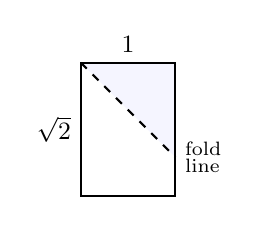
\begin{tikzpicture}[font=\small, baseline=(current bounding box.north)]
  \pgfmathsetmacro{\w}{1.2}
  \pgfmathsetmacro{\h}{1.2*sqrt(2)}
  \fill[blue!4] (0,\h) -- (\w,\h) -- (\w,\h-\w) -- cycle;
  \draw[thick] (0,0) rectangle (\w,\h);
  \draw[dashed, thick] (0,\h) -- (\w,\h-\w);
  \node[above] at (\w/2,\h) {$1$};
  \node[left] at (0,\h/2) {$\sqrt{2}$};
  \node[right, font=\scriptsize, align=left] at (\w,\h-\w)
    {fold\\[-2pt]line};
\end{tikzpicture}
\end{minipage}

\end{enumerate}

\newpage

% ================================================================
% PAGE 3: new rules, new ratios, and other shapes
% ================================================================

\parttitle{2}{New rules, new ratios}

Each new rule for cutting a rectangle leads to a new ratio.

\begin{enumerate}[resume]

% Answers: whole card 1 : x; one strip x/3 : 1. Times 3: x : 3, divide
% by x: 1 : 3/x.
% Same shape, so 1 : x = 1 : 3/x and x = 3/x. Times x: x^2 = 3. Square
% root: x = sqrt(3). The card is 1 : sqrt(3), about 1 : 1.732.
\item A card can be cut into three equal strips, each similar to the whole
card. The long side of the card is $x$. Find the ratio of the card, short :
long.

\vspace{3pt}
\begin{minipage}[t]{0.30\linewidth}
\vspace{0pt}
\cutdiagram{3}{1.732}{$x$}{$?$}{cut}
\end{minipage}%
\begin{minipage}[t]{0.66\linewidth}
\vspace{2pt}
{\renewcommand{\arraystretch}{2}
\begin{tabular}{@{}l@{\qquad}l@{}}
Whole card, short : long & \ansline[1.4cm]\ $:$\ \ansline[1.4cm]\\
One strip, short : long  & \ansline[1.4cm]\ $:$\ \ansline[1.4cm]\\
\end{tabular}}
\end{minipage}

\vspace{2cm}
The card is $1:{}$\gap.

% Answers: (a) one strip x/5 : 1 = 1 : 5/x, so x = 5/x, x^2 = 5 and the
% card is 1 : sqrt(5). (b) 1 : sqrt(n). (c) n must be a square number.
% For n = 4 the card is 1 : 2: cut into 4 strips, each strip is
% 1/2 : 1 = 1 : 2.
\item
\begin{enumerate}
  \item A card can be cut into five equal strips, each similar to the whole
        card. Find its ratio short : long.
  \item Write down the ratio for a card that cuts into $n$ similar strips in
        the same way.
  \item For which values of $n$ can the ratio be written with whole numbers?
        Draw an example, cut into its strips.
\end{enumerate}

% Answers: (a) left over (x - 1) : 1; divide by (x - 1): 1 : 1/(x - 1).
% (b) Same shape, so x = 1/(x - 1). Times (x - 1): x^2 - x = 1, so
% x^2 - x - 1 = 0. (c) (x - 1/2)^2 - 5/4 = 0. Add 5/4:
% (x - 1/2)^2 = 5/4. Square root (x is positive, so take the positive
% root): x - 1/2 = sqrt(5)/2. Add 1/2: x = (1 + sqrt(5))/2 = 1.618.
% The golden rectangle is 1 : (1 + sqrt(5))/2, about 1 : 1.618.
\item
\begin{minipage}[t]{0.74\linewidth}
A rectangle is $1:x$. Cutting off the largest possible square leaves a
rectangle similar to the whole rectangle. This is the \textbf{golden
rectangle}.
\begin{enumerate}
  \item Fill in the gaps.

        \vspace{1pt}
        \begin{minipage}[t]{0.6\linewidth}
        \centering
        \worktitle{Left over, short : long}
        \bothsides{\eqgap \& : \& 1\\ 1 \& : \& \eqgap\\}{\div(x-1)}
        \end{minipage}
  \item Show that $x^2-x-1=0$.
  \item Use the fact $x^2-x-1=\left(x-\frac{1}{2}\right)^2-\frac{5}{4}$ to
        solve the equation by rearranging. Give the ratio of the golden
        rectangle exactly and to 3 decimal places.
\end{enumerate}
\end{minipage}\hfill
\begin{minipage}[t]{0.22\linewidth}
\vspace{6pt}
\centering
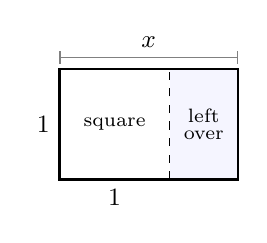
\begin{tikzpicture}[font=\small, baseline=(current bounding box.north)]
  \pgfmathsetmacro{\s}{1.4}
  \pgfmathsetmacro{\g}{1.4*1.618}
  \fill[blue!4] (\s,0) rectangle (\g,\s);
  \draw[thick] (0,0) rectangle (\g,\s);
  \draw[dashed] (\s,0) -- (\s,\s);
  \node[left] at (0,\s/2) {$1$};
  \node[below] at (\s/2,0) {$1$};
  \draw[|-|, gray] (0,\s+0.15) -- node[above, text=black] {$x$} (\g,\s+0.15);
  \node[font=\scriptsize] at (\s/2,\s/2) {square};
  \node[font=\scriptsize, align=center] at ({(\s+\g)/2},\s/2)
    {left\\[-2pt]over};
\end{tikzpicture}
\end{minipage}

% Answers: (a) (sqrt(2) - 1) : 1. (b) Multiply both parts by
% sqrt(2) + 1: (sqrt(2) - 1)(sqrt(2) + 1) = 2 + sqrt(2) - sqrt(2) - 1 = 1,
% so the left over rectangle is 1 : (sqrt(2) + 1).
% (c) Cutting two squares off a 1 : (1 + sqrt(2)) rectangle leaves
% (1 + sqrt(2) - 2) : 1 = (sqrt(2) - 1) : 1, which is 1 : (1 + sqrt(2))
% by (b), so it is similar. (1 + sqrt(2) = 2.414... is the silver ratio.)
\item
\begin{minipage}[t]{0.74\linewidth}
The largest possible square is cut off a sheet of A4, $1:\sqrt{2}$.
\begin{enumerate}
  \item Write the rectangle left over as short : long.
  \item Fill in the gaps. (Hint: work out
        $\left(\sqrt{2}-1\right)\left(\sqrt{2}+1\right)$.)

        \vspace{1pt}
        \begin{minipage}[t]{0.6\linewidth}
        \centering
        \worktitle{Left over, short : long}
        \bothsides{\sqrt{2}-1 \& : \& 1\\ \eqgap \& : \& \eqgap\\}
          {\times\left(\sqrt{2}+1\right)}
        \end{minipage}
  \item A rectangle is $1:\left(1+\sqrt{2}\right)$. Show that cutting off two
        squares leaves a rectangle similar to the whole rectangle.
\end{enumerate}
\end{minipage}\hfill
\begin{minipage}[t]{0.22\linewidth}
\vspace{6pt}
\centering
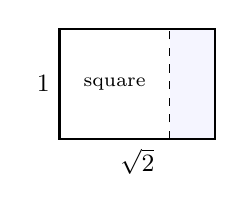
\begin{tikzpicture}[font=\small, baseline=(current bounding box.north)]
  \pgfmathsetmacro{\s}{1.4}
  \pgfmathsetmacro{\g}{1.4*sqrt(2)}
  \fill[blue!4] (\s,0) rectangle (\g,\s);
  \draw[thick] (0,0) rectangle (\g,\s);
  \draw[dashed] (\s,0) -- (\s,\s);
  \node[left] at (0,\s/2) {$1$};
  \node[below] at (\g/2,0) {$\sqrt{2}$};
  \node[font=\scriptsize] at (\s/2,\s/2) {square};
\end{tikzpicture}
\end{minipage}

\end{enumerate}

\parttitle{3}{Other shapes}

\begin{enumerate}[resume]

% Answers: (a) The whole triangle has hypotenuse sqrt(2) and each piece
% has hypotenuse 1, so piece : whole = 1 : sqrt(2), the same as A4.
% (b) Each piece has 1/3 of the area, so the area scale factor is 1/3
% and the length scale factor is 1/sqrt(3): 1 : sqrt(3), the same as
% Q9. (c) In the 4 by 4 grid, the four L-shapes are the squares
% {(0,0),(1,0),(0,1)}, {(1,1),(2,1),(1,2)}, {(2,0),(3,0),(3,1)} and
% {(0,2),(0,3),(1,3)}, counting from the bottom left; 1 : 2.
% (d) Hint: the area is multiplied by k^2.
% Each piece has area 1/n of the whole shape, so the area scale
% factor is 1/n and the length scale factor is 1/sqrt(n), giving
% 1 : sqrt(n). For A4, n = 2 gives 1 : sqrt(2) without solving an
% equation.
\item Each shape is cut into equal pieces, and each piece is similar to the
whole shape. Find the ratio of lengths, piece : whole.

\vspace{2pt}
\begin{minipage}[b]{0.31\linewidth}
\centering
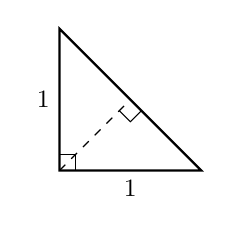
\begin{tikzpicture}[font=\small]
  \pgfmathsetmacro{\a}{1.8}
  \draw[thick] (0,0) -- (\a,0) -- (0,\a) -- cycle;
  \draw[dashed] (0,0) -- (\a/2,\a/2);
  \draw (0.2,0) -- (0.2,0.2) -- (0,0.2);
  \draw ({\a/2-0.14},{\a/2-0.14}) -- ({\a/2},{\a/2-0.28})
    -- ({\a/2+0.14},{\a/2-0.14});
  \node[below] at (\a/2,0) {$1$};
  \node[left] at (0,\a/2) {$1$};
\end{tikzpicture}

\small (a) Two pieces
\end{minipage}\hfill
\begin{minipage}[b]{0.36\linewidth}
\centering
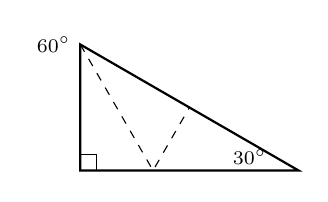
\begin{tikzpicture}[font=\small]
  \pgfmathsetmacro{\s}{1.6}
  \coordinate (C) at (0,0);
  \coordinate (A) at ({\s*sqrt(3)},0);
  \coordinate (B) at (0,\s);
  \coordinate (D) at ({\s/sqrt(3)},0);
  \coordinate (E) at ({\s*sqrt(3)/2},{\s/2});
  \draw[thick] (C) -- (A) -- (B) -- cycle;
  \draw[dashed] (B) -- (D) -- (E);
  \draw (0.2,0) -- (0.2,0.2) -- (0,0.2);
  \node[font=\scriptsize] at ({\s*sqrt(3)-0.62},0.17) {$30^\circ$};
  \node[font=\scriptsize, left] at (B) {$60^\circ$};
\end{tikzpicture}

\small (b) Three pieces
\end{minipage}\hfill
\begin{minipage}[b]{0.31\linewidth}
\centering
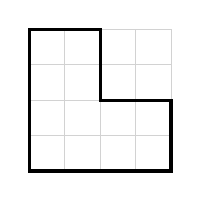
\begin{tikzpicture}[scale=0.45]
  \draw[gray!35] (0,0) grid (4,4);
  \draw[very thick] (0,0) -- (4,0) -- (4,2) -- (2,2) -- (2,4) -- (0,4) -- cycle;
\end{tikzpicture}

\small (c) Four pieces: draw them
\end{minipage}

\begin{enumerate}
  \setcounter{enumii}{3}
  \item A shape is cut into $n$ equal pieces like this. Explain why the ratio
        of lengths, piece : whole, is $1:\sqrt{n}$. Use this to explain why A4
        is $1:\sqrt{2}$ in a different way.

        Fill in the hint first: if every length is multiplied by $k$, then the
        area is \ansline[3.5cm].
\end{enumerate}

\end{enumerate}

\newpage

% ================================================================
% PAGE 4: more dimensions, and patterns
% ================================================================

\parttitle{4}{More dimensions, and patterns}

\begin{enumerate}[resume]

% Answers: (a) half block z/2 : 1 : y; times 2: z : 2 : 2y; divide by z:
% 1 : 2/z : 2y/z. (b) Same shape, so 1 : y : z = 1 : 2/z : 2y/z. So
% y = 2/z, which gives z = 2/y, and z = 2y/z, which gives z^2 = 2y.
% Then 4/y^2 = 2y, so y^3 = 2. (c) y = cbrt(2) = 1.260, z = 2/y =
% cbrt(4) = 1.587: 1 : cbrt(2) : cbrt(4), about 1 : 1.260 : 1.587.
% (d) Edges a, a cbrt(2), a cbrt(4), volume 2a^3 = 1000, a^3 = 500,
% a = 7.94 cm. The middle edge is a cbrt(2) = cbrt(1000) = 10 cm exactly,
% and the longest edge is cbrt(2000) = 12.60 cm.
\item A block of cheese is a cuboid with edges $1:y:z$, from shortest to
longest. Halving its longest edge cuts it into two blocks similar to the whole
block.

\begin{minipage}[t]{0.66\linewidth}
\begin{enumerate}
  \item Fill in the gaps.

        \vspace{1pt}
        \begin{center}
        \worktitle{Half block, shortest : middle : longest}
        \bothsides[ratio3]{\eqgap \& : \& 1 \& : \& y\\
          \eqgap \& : \& \eqgap \& : \& \eqgap\\
          1 \& : \& \eqgap \& : \& \eqgap\\}{\times2, \div z}
        \end{center}
  \item The blocks are similar, so $1:y:z$ is equal to your last line. Use
        this to show that $y^3=2$.
\end{enumerate}
\end{minipage}\hfill
\begin{minipage}[t]{0.30\linewidth}
\vspace{4pt}
\centering
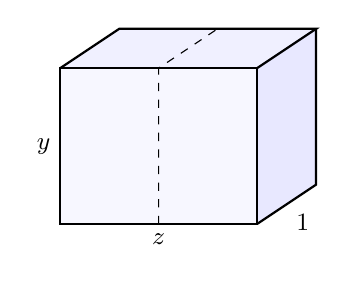
\begin{tikzpicture}[font=\small, baseline=(current bounding box.north)]
  \pgfmathsetmacro{\Z}{2.5}
  \pgfmathsetmacro{\Y}{1.98}
  \pgfmathsetmacro{\dx}{0.75}
  \pgfmathsetmacro{\dy}{0.5}
  \fill[blue!3] (0,0) rectangle (\Z,\Y);
  \fill[blue!6] (0,\Y) -- (\dx,\Y+\dy) -- (\Z+\dx,\Y+\dy) -- (\Z,\Y) -- cycle;
  \fill[blue!9] (\Z,0) -- (\Z+\dx,\dy) -- (\Z+\dx,\Y+\dy) -- (\Z,\Y) -- cycle;
  \draw[thick] (0,0) rectangle (\Z,\Y);
  \draw[thick] (0,\Y) -- (\dx,\Y+\dy) -- (\Z+\dx,\Y+\dy) -- (\Z,\Y);
  \draw[thick] (\Z,0) -- (\Z+\dx,\dy) -- (\Z+\dx,\Y+\dy);
  \draw[dashed] (\Z/2,0) -- (\Z/2,\Y) -- (\Z/2+\dx,\Y+\dy);
  \node[below] at (\Z/2,0) {$z$};
  \node[left] at (0,\Y/2) {$y$};
  \node[below right] at (\Z+\dx/2,\dy/2) {$1$};
\end{tikzpicture}
\end{minipage}

\begin{enumerate}
  \setcounter{enumii}{2}
  \item Find the ratio $1:y:z$ exactly and to 3 decimal places.
  \item A block has a volume of $1$ litre ($1000\text{ cm}^3$). Find its
        edges, and show that one is $10$\,cm.
\end{enumerate}

% Answers: (a) half box c/2 : 1 : a : b = 1 : 2/c : 2a/c : 2b/c.
% (b) Same shape, so a = 2/c, b = 2a/c = a x a = a^2 and
% c = 2b/c = a x b = a^3. Then a = 2/c = 2/a^3, so a^4 = 2.
% (c) a = 2^(1/4): 1 : 1.189 : 1.414 : 1.682. 1.189 m = 1189 mm is the
% long side of A0 in Q6: the long side of A0 is sqrt(2) x, where
% x^2 = 1/sqrt(2), and this is the fourth root of 2 metres.
\item We cannot draw a \textbf{four-dimensional box}, but we can describe one:
it has four edges, each at right angles to all the others. One has edges
$1:a:b:c$, from shortest to longest. Halving its longest edge gives two boxes
similar to the whole box.
\begin{enumerate}
  \item Write the half box, shortest : \ldots : longest, in the form
        $1:\ldots:\ldots:\ldots$
  \item Show that $b=a^2$ and $c=a^3$, and that $a^4=2$.
  \item Find the ratio $1:a:b:c$ to 3 decimal places. One of these numbers
        appears earlier on this sheet. Where, and why?
\end{enumerate}

% Answers: (a) Columns 2D, 3D, 4D, d dimensions. 2 slices: sqrt(2),
% cbrt(2), 2^(1/4), 2^(1/d). 3 slices: sqrt(3), cbrt(3), 3^(1/4),
% 3^(1/d). n slices: sqrt(n), cbrt(n), n^(1/4), n^(1/d); r^d = n.
% (b) 2D sqrt(2) = 1.414, 3D cbrt(4) = 1.587, 4D 2^(3/4) = 1.682,
% 10D 2^(9/10) = 1.866. (c) longest / shortest = r^(d-1) = r^d / r = 2/r.
% As d grows, r gets closer to 1, so the answer gets closer to 2. It is
% always less than 2 because r is more than 1.
\item A rectangle, box or four-dimensional box is cut into equal slices across
its longest edge, and each slice is similar to the whole shape. Its edges are
then in the ratio $1:r:r^2:\ldots$
\begin{enumerate}
  \item Complete the table of the values of $r$. Some of them have been found
        already on this sheet.

        \vspace{1pt}
        {\small\renewcommand{\arraystretch}{1.3}
        \begin{tabular}{|l|*{4}{C{2.75cm}|}}
        \hline
        & \textbf{Rectangle (2D)} & \textbf{Box (3D)} & \textbf{4D box}
          & \textbf{$d$ dimensions}\\ \hline
        \textbf{2 slices} & $\sqrt{2}$ & & & \\ \hline
        \textbf{3 slices} & & & & \\ \hline
        \textbf{$n$ slices} & & & & \\ \hline
        \end{tabular}}
  \item For 2 slices, work out longest edge $\div$ shortest edge in 2, 3, 4
        and 10 dimensions.
  \item What happens to longest edge $\div$ shortest edge as the number of
        dimensions gets larger? Explain why it is always less than $2$.
        (Hint: $r^{d-1}=r^d\div r$.)
\end{enumerate}

% Answers: (a) 1/2 + 1/4 + 1/8 + 1/16 + 1/32 + 1/64 = 63/64 m^2.
% (b) The sheet left over at each step gets smaller and smaller, so the
% total area gets closer and closer to the whole sheet of A0, 1 m^2.
% (c) (1/sqrt(2))^2 = 1/2, so (1/sqrt(2))^10 = (1/2)^5 = 1/32.
% 841/32 = 26.3 and 1189/32 = 37.2, so A10 is 26 mm by 37 mm.
\item
\begin{minipage}[t]{0.64\linewidth}
The diagram shows a sheet of A0 cut into one sheet of each size from A1 to
A6, with one more sheet of A6 left over.
\begin{enumerate}
  \item What is the total area of the sheets from A1 to A6, in m$^2$?
  \item The pattern carries on forever, to A7, A8, A9 and so on. What happens
        to the total area of all the sheets? Explain why.
  \item For lengths, A0 : A10 $=1:\left(\frac{1}{\sqrt{2}}\right)^{10}$. Show
        that this is $1:\frac{1}{32}$, and find the size of A10.
\end{enumerate}
\end{minipage}\hfill
\begin{minipage}[t]{0.33\linewidth}
\vspace{2pt}
\centering
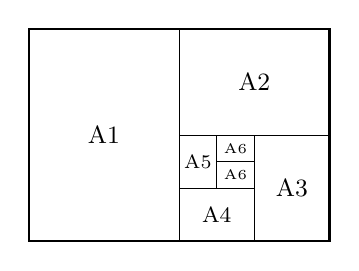
\begin{tikzpicture}[font=\small, baseline=(current bounding box.north)]
  \pgfmathsetmacro{\H}{2.7}
  \pgfmathsetmacro{\W}{2.7*sqrt(2)}
  \draw[thick] (0,0) rectangle (\W,\H);
  \draw (\W/2,0) -- (\W/2,\H);
  \draw (\W/2,\H/2) -- (\W,\H/2);
  \draw (3*\W/4,0) -- (3*\W/4,\H/2);
  \draw (\W/2,\H/4) -- (3*\W/4,\H/4);
  \draw (5*\W/8,\H/4) -- (5*\W/8,\H/2);
  \draw (5*\W/8,3*\H/8) -- (3*\W/4,3*\H/8);
  \node at (\W/4,\H/2) {A1};
  \node at (3*\W/4,3*\H/4) {A2};
  \node at (7*\W/8,\H/4) {A3};
  \node[font=\footnotesize] at (5*\W/8,\H/8) {A4};
  \node[font=\scriptsize] at (9*\W/16,3*\H/8) {A5};
  \node[font=\tiny] at (11*\W/16,7*\H/16) {A6};
  \node[font=\tiny] at (11*\W/16,5*\H/16) {A6};
\end{tikzpicture}
\end{minipage}

% Answers: (a) Cutting k squares off a 1 : x rectangle leaves
% (x - k) : 1 = 1 : 1/(x - k), so x = 1/(x - k), x^2 - kx = 1 and
% x^2 - kx - 1 = 0. (b) (x - 3/2)^2 - 13/4 = 0, so (x - 3/2)^2 = 13/4,
% x - 3/2 = sqrt(13)/2 and x = (3 + sqrt(13))/2 = 3.303: 1 : 3.303.
% (c) (x - k/2)^2 = (k^2 + 4)/4, x - k/2 = sqrt(k^2 + 4)/2, so
% x = (k + sqrt(k^2 + 4))/2. k = 1 gives (1 + sqrt(5))/2 and k = 2 gives
% (2 + sqrt(8))/2 = 1 + sqrt(2). (d) Open.
\item A rectangle is $1:x$. Cutting off $k$ squares leaves a similar
rectangle. (Q11 is $k=1$ and Q12 is $k=2$.)
\begin{enumerate}
  \item Show that $x^2-kx-1=0$.
  \item Use the fact
        $x^2-kx-1=\left(x-\frac{k}{2}\right)^2-\frac{k^2+4}{4}$ to solve
        $x^2-3x-1=0$ by rearranging. Give the ratio when $k=3$, exactly and to
        3 decimal places.
  \item Rearrange $\left(x-\frac{k}{2}\right)^2-\frac{k^2+4}{4}=0$ to find
        $x$ in terms of $k$. Check it with Q11 and Q12.
  \item Invent your own rule for cutting a rectangle, a triangle or a box into
        pieces, so that one or more of the pieces is similar to the whole
        shape. Find the ratio that your rule leads to.
\end{enumerate}

\end{enumerate}

\end{document}
